\chapter{Core Implementation}

%-------------------------------------------------------------------------------------------------------

\section{Building the Project}

\subsection{Obtaining the Source}
\noindent 
The latest version of the project's source code can be checked out via \textit{git} using: \\

\indent \textit{git clone https://github.com/swordmaster2k/botnav.git} \\

\noindent
Or downloaded as a ZIP file from \url{https://github.com/swordmaster2k/botnav}. \\ 

\noindent
Alternatively the most up to date version at the time of printing is available on the CD at the front of this thesis.

\subsection{Compiling the D* Lite Cython Module}
\noindent
The planning algorithm D* Lite must be compiled as a Cython module, the original source code was provided by Maxim Likhachev of CMU and Sven Koenig of USC in C. It has been modified to make it compatible with the core Python system using Cython, as Python is implemented in C \cite{•} it is inherently compatible with the sample of D* Lite that is provided by its authors.

\noindent
To build D* Lite you will need Python3.4, the Python3.4 headers, gcc, and make. It \textbf{must} be built for each platform on which it will execute as C compiles to machine code making it \textit{target dependent}. From a terminal navigate to the source code directory \textit{BotNav/algorithm/dstarlite\_build/}. \\

\noindent
The make file contains two build rules:
\begin{enumerate}
\item \textit{make} - \indent which builds the module \textit{dstarlite\_c.so} 
\item \textit{make clean} - \indent cleans all previous output files from the build process \\
\end{enumerate}

\noindent
Once the module file \textit{dstarlite\_c.so} has been successfully built for the target platform it can simply be dropped into the parent directory \textit{BotNav/algorithm/}. The Python source code contains a reference to the module and will automatically link it in at execution time. 

\subsection{Running it in Python3}
\noindent
By default the project is set-up to run a sample simulation with \textit{sample.map} using the GridNav path planning algorithm. It will output the results of its run to the \textit{BotNav/maps/output/} directory and is configured to compute a path from every traversable cell to the goal. To run it simply navigate to the path containing \textit{tester.py} and type: \\

\indent \textit{python3 tester.py config.botnav} \\

\noindent
The argument passed to \textit{tester.py} is the path to the default configuration file, the contents of which will be discussed later in this chapter. After running the above command in a terminal the result shall look similar to Figure \ref{sample_output}.

\begin{figure}[htbp]

\center 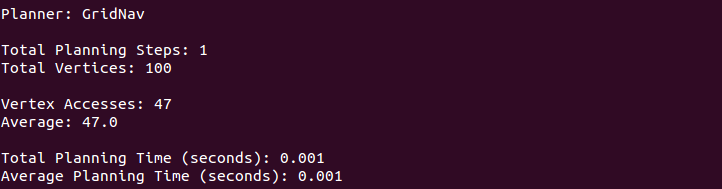
\includegraphics[width=435pt]{illustrations/sample_output}\\
\caption{An example of the type of output generated after running GridNav over \textit{sample.map} in simulation mode.} 
\label{sample_output}

\end{figure}

%-------------------------------------------------------------------------------------------------------

\section{Running Simulations}
\noindent
Simulations provide an easy means of testing each planning algorithm in controllable environments, it speeds up the testing process immeasurably, and provides reproduce-able results. The most powerful feature of simulations is the ability to plan a path from every free cell in the environment, the result of each traversal is placed into a separate timestamped folder. This data can then be easily mined and analysed in order to gauge how each algorithm performed for a particular scenario.

\subsection{Configuration}
\noindent 
When carrying out simulated runs three parameters must be set in the corresponding configuration file they are \textit{map}, \textit{mode}, and \textit{planner}. Below is an example of the configuration required to run a simulated trial using D* Lite: \\

	\indent \textit{map=maps/simple.map \\}
	\indent \textit{planner=d\_star\_lite \\}
	\indent \textit{mode=simulated \\}

\noindent
The most important parameter setting here is \textit{mode} which is set to simulated. At run time this informs the \textit{Tester} class that we want to run an experimental simulation across all traversable cells and that we do not need a communications channel via \textit{Proxy}.

%-------------------------------------------------------------------------------------------------------

\section{Using a Real Bot}
\noindent
The real test for any path planning algorithm is its practical effectiveness and the only way to gauge this is using a physical robotic platform i.e.``a Real Bot''. The simulations that we have performed here are very limited in nature as they do not take into account any variability in the mechanics of the robot. \\
  
Mention how using a real robot differs by:

\begin{itemize}
\item The need for communications.
\item Introducing drift wheel slippage etc.
\item By proving the practical application of the planner.
\end{itemize}

\subsection{Configuration}
Outline the changes that need to be made to the configuration file, highlight the fact that communications medium is required USB, Bluetooth, or Wifi. Explain the different variations.

%-------------------------------------------------------------------------------------------------------

\section{How the Planner Works}
Explain how the planner was implemented in code, the control logic, looping structure, reacting to change, and the conditions for terminating the planner.

\subsection{Five Simple Steps}
Every planner in robotics splits the problem into five simple steps, include them under this section as numbered items. State any recursive operations that take place. Also include a flowchart or diagram in some form.

\subsection{Abstracting Away from the Algorithm}
This section will cover the abstract model that the Algorithm class enforces, every planning algorithm has a common interface which allows them to be interchanged. Explain how this is achieved using abstraction and talk about the advantages.

%-------------------------------------------------------------------------------------------------------

\section{Open Field D*}
Core of the project very important, state that every implementation of Field D* to date is closed source NASA's code is not available, nor is Carnegie Mellon's. Open Field D* is significant because it bucks this trend making it open to ITB students and others.

\subsection{Modifying D* Lite}
Point out the key differences between D* Lite and Field D* from a coding perspective, nodes to cell corners how this is represented, linear interpolation. Using Georgia Institute of Technologies D* Lite code state the modifications required to get Field D*.

\subsection{Basic Implementation}
Cover basic implementation of Field D*, most importantly state any problems encountered, or variations/optimisations made during the coding stage.

%-------------------------------------------------------------------------------------------------------